\section{\textit{Benchmark}}
Seguono i risultati dei \textit{benchmark} effettuati dal team di sviluppo di TimescaleDB, che confrontano
le prestazioni dei due strumenti.

\begin{center}
	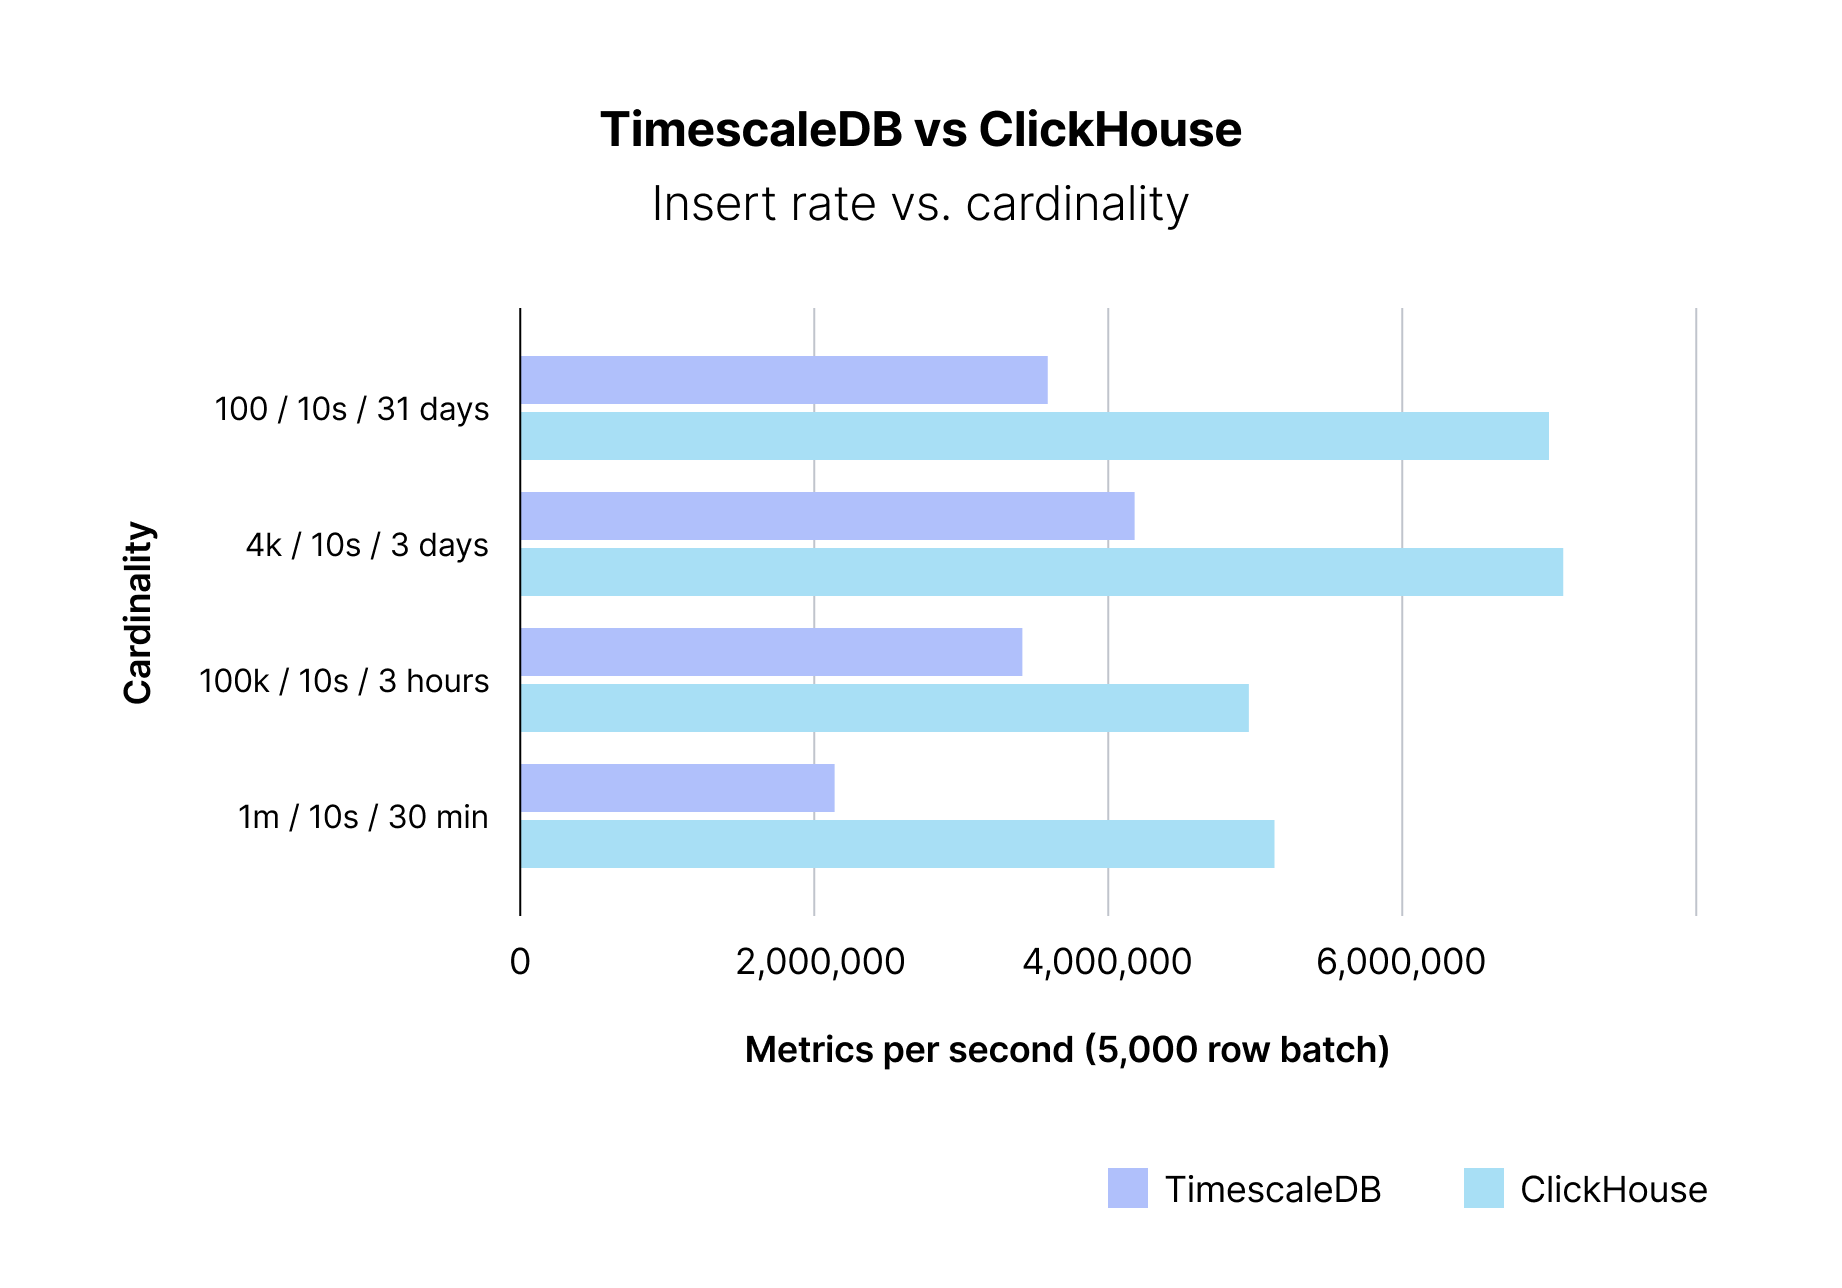
\includegraphics[width=0.85\textwidth]{imgs/01-timescale-vs-clickhouse.png}
	\captionof{figure}{\href{https://www.timescale.com/blog/what-is-clickhouse-how-does-it-compare-to-postgresql-and-timescaledb-and-how-does-it-perform-for-time-series-data/}{ClickHouse ha performance migliori di TimescaleDB con batch di dimensione superiore a 5,000 righe}}
\end{center}

\begin{center}
	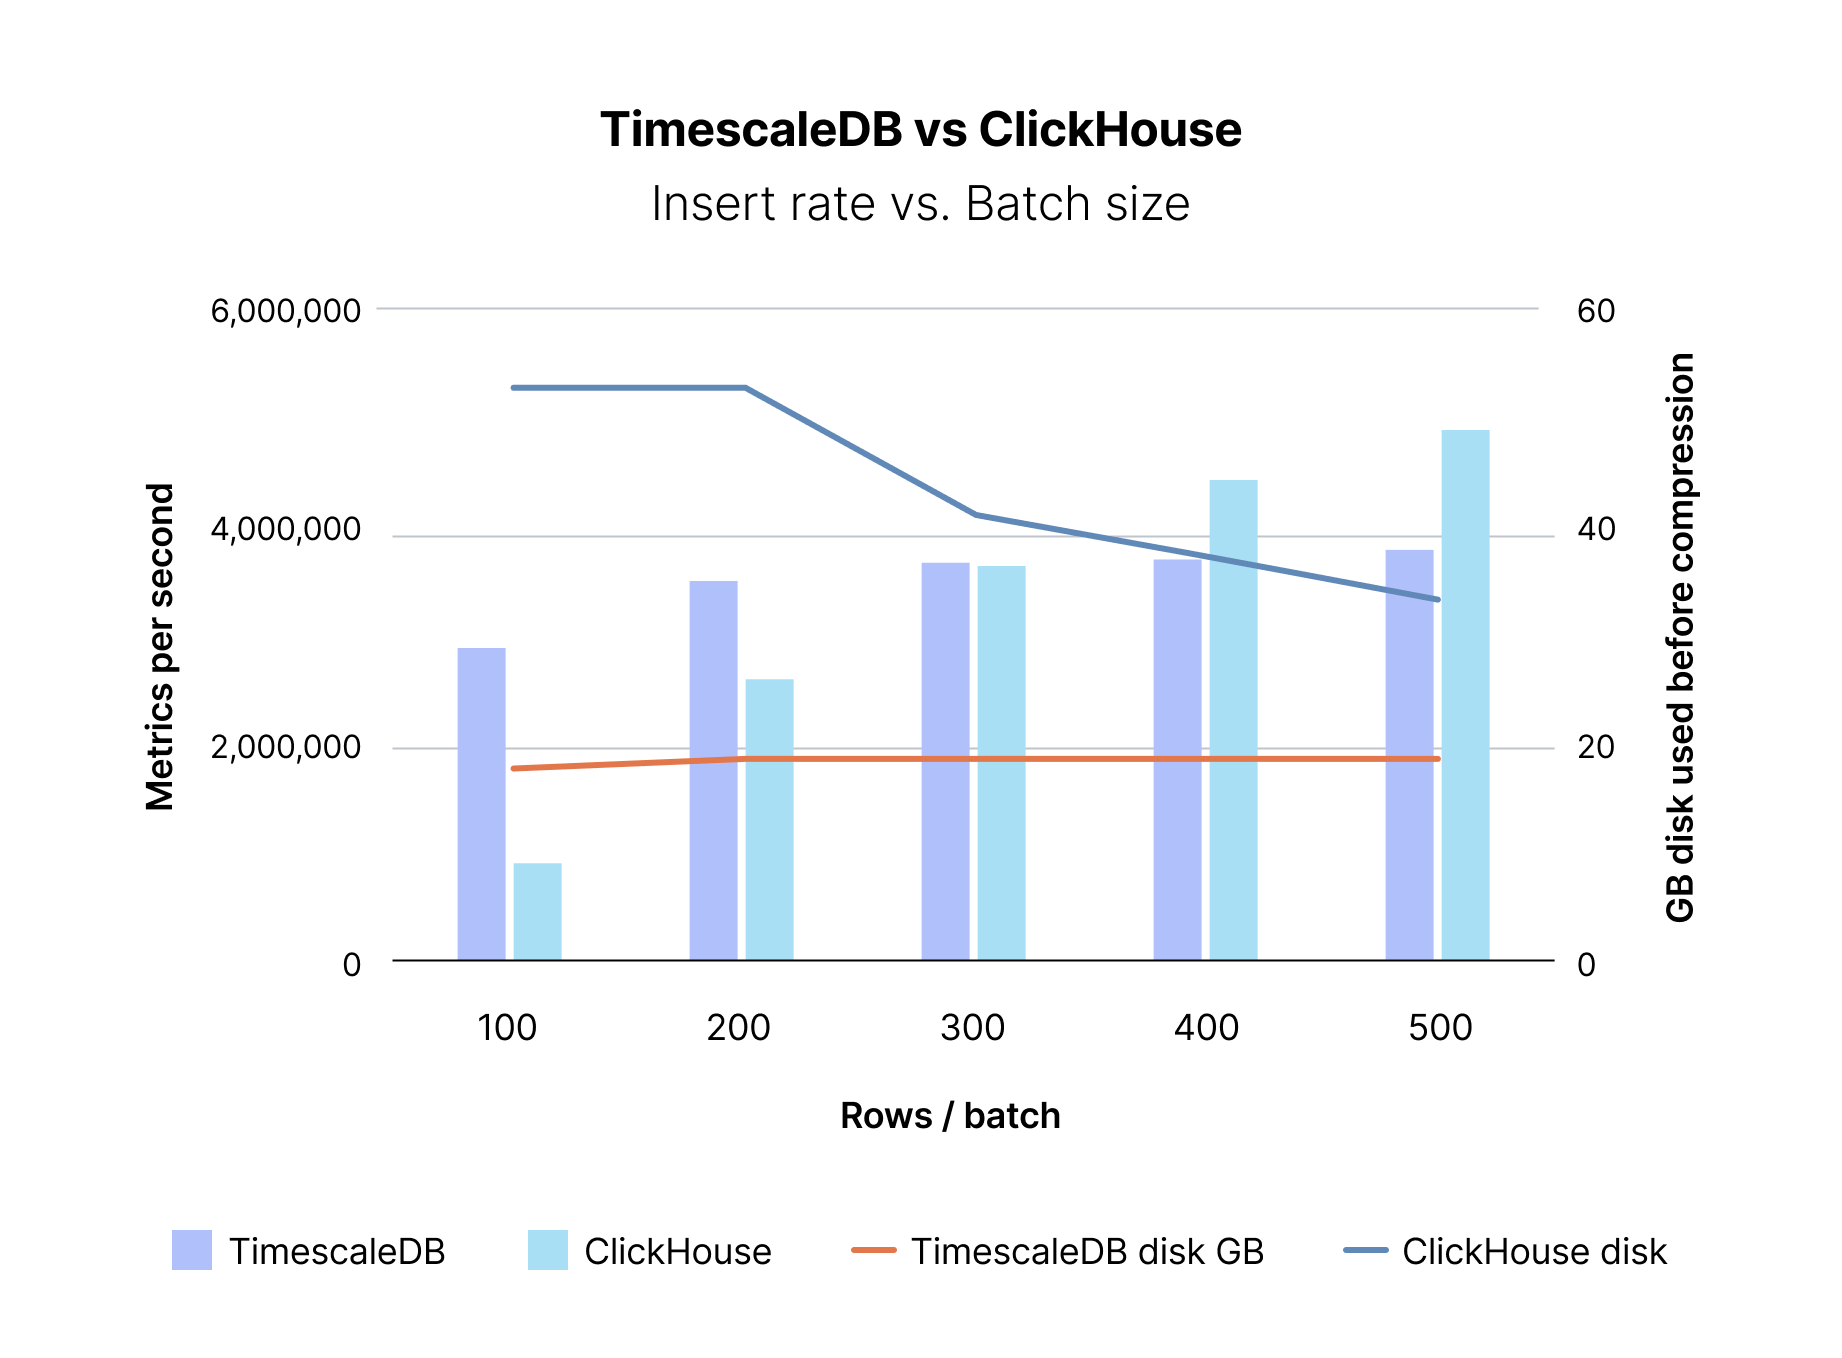
\includegraphics[width=0.85\textwidth]{imgs/02-small-batch-insert-performance.png}
	\captionof{figure}{\href{https://www.timescale.com/blog/what-is-clickhouse-how-does-it-compare-to-postgresql-and-timescaledb-and-how-does-it-perform-for-time-series-data/}{Timescale ha performance migliori di ClickHouse con batch di dimensione più contenuta e usa una quantità di disco inferiore di 2.7 volte}}
\end{center}

\begin{center}
	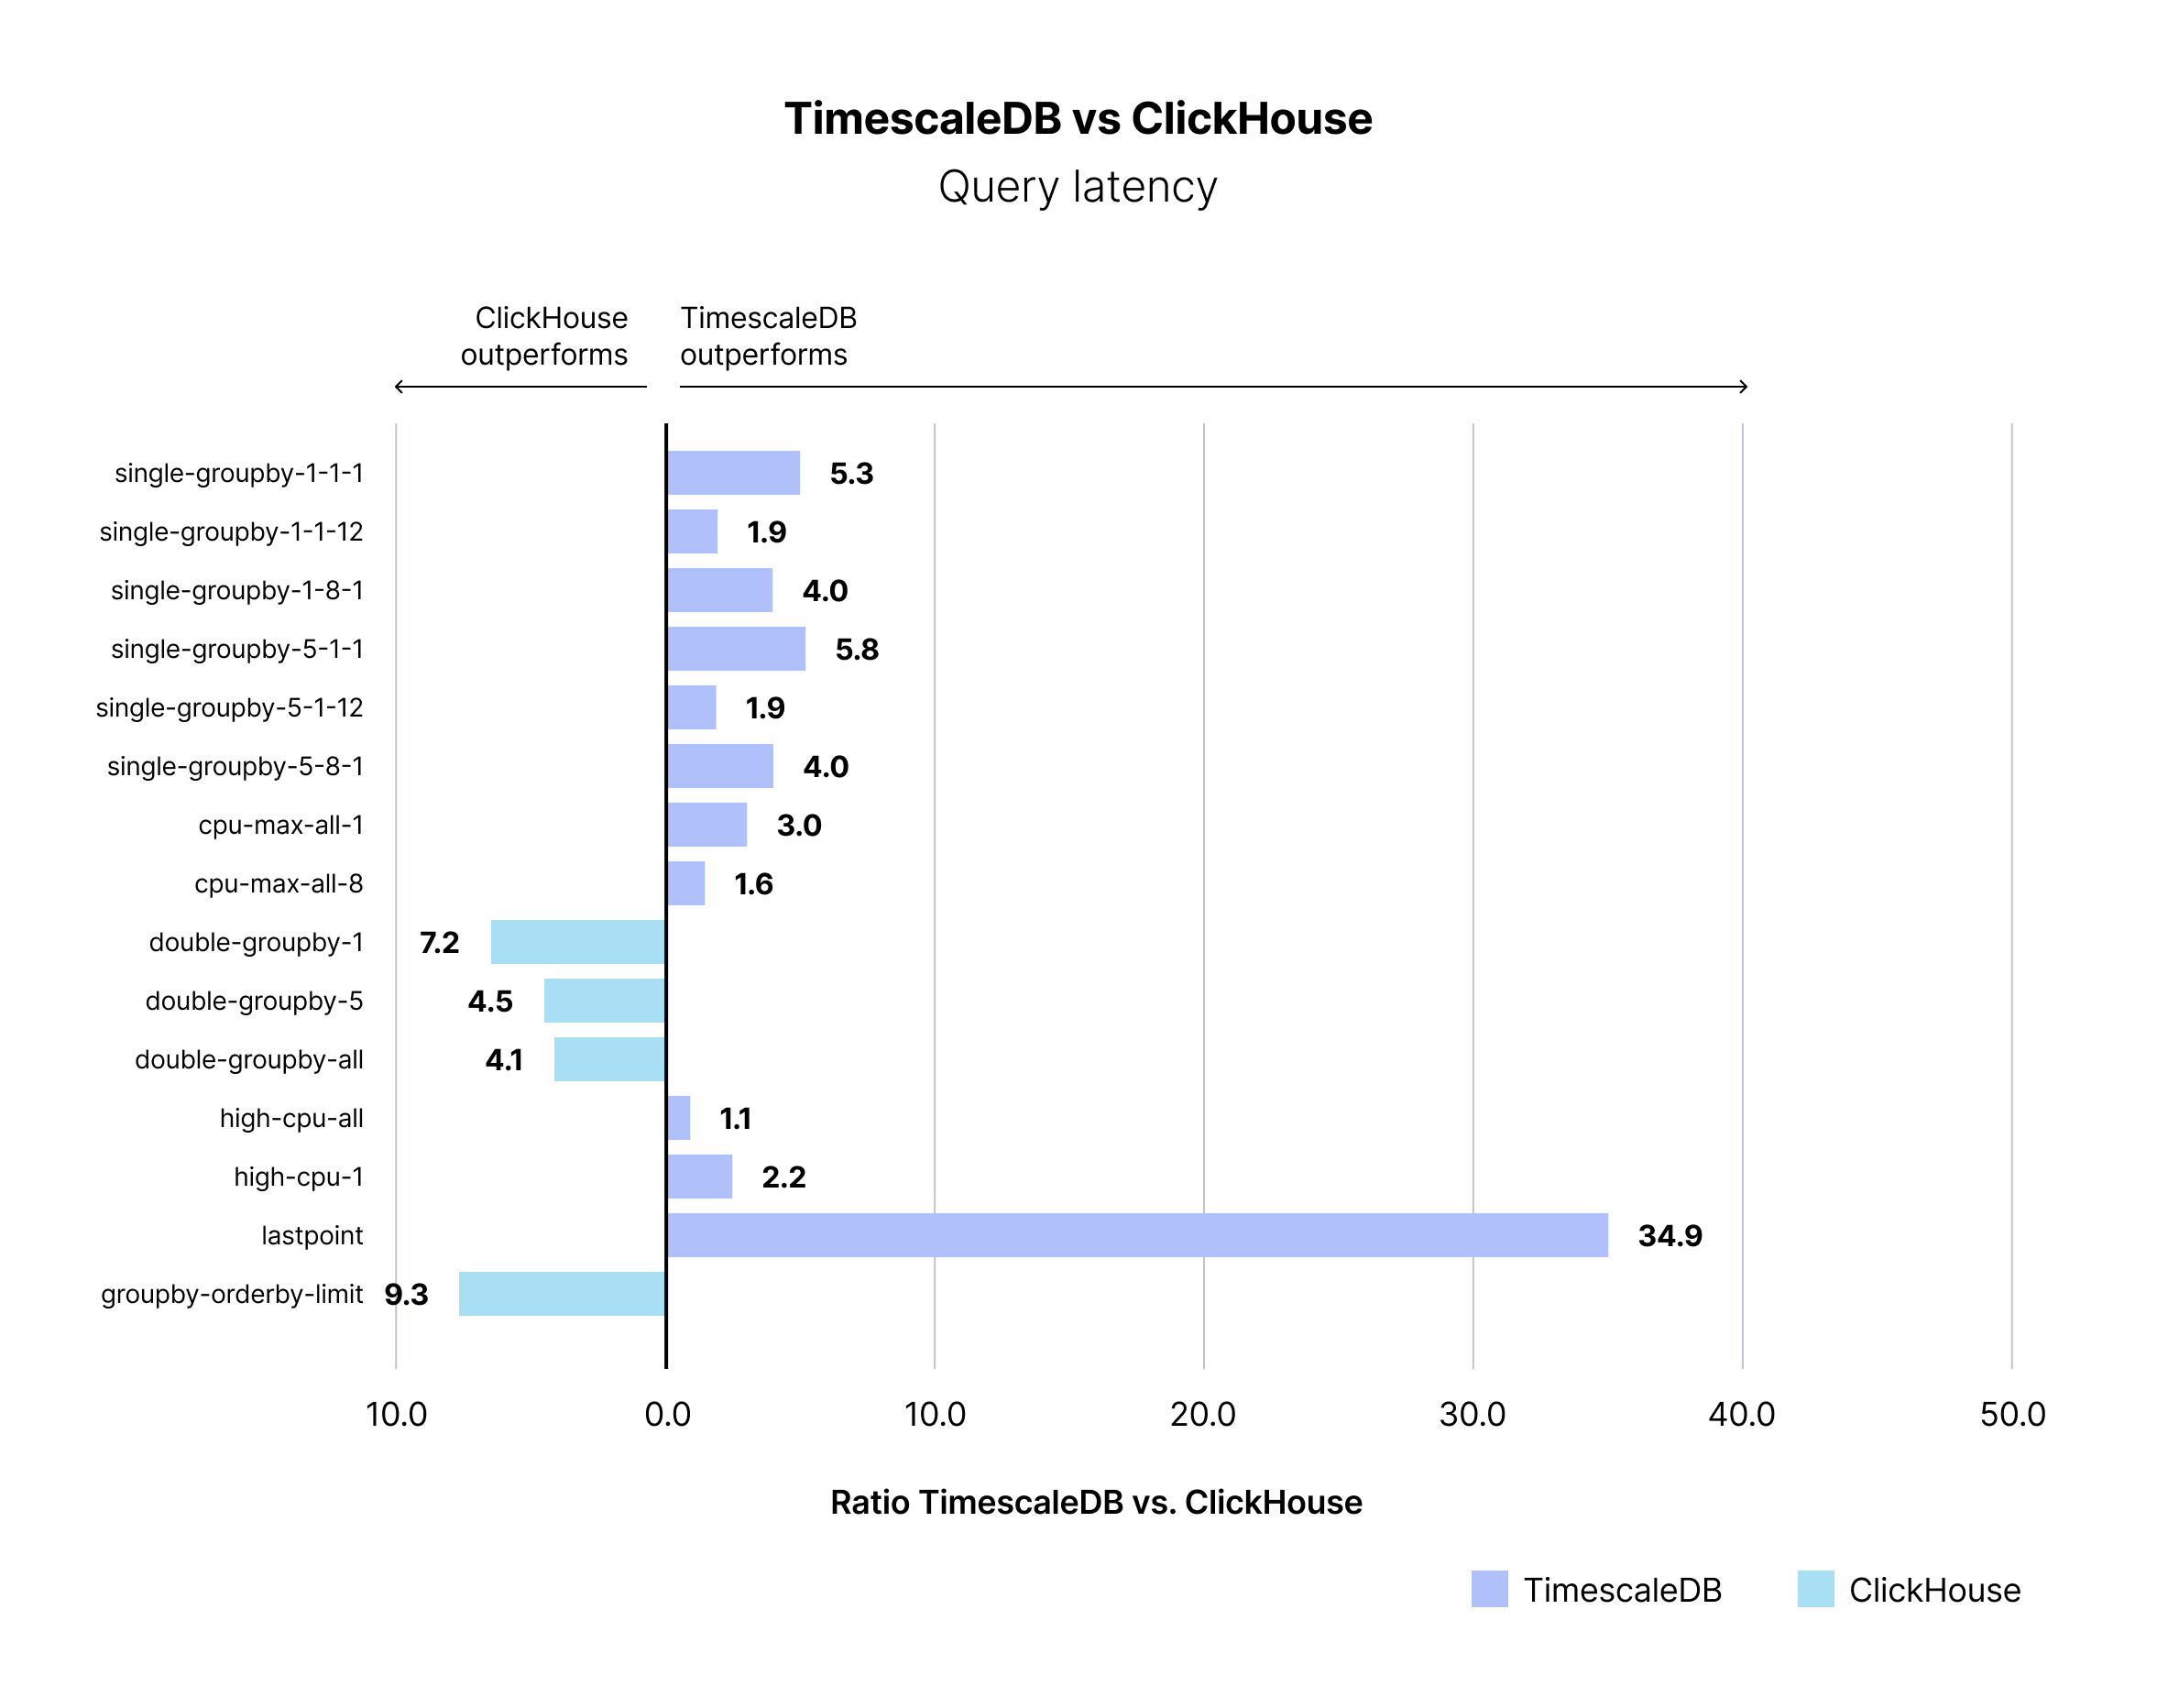
\includegraphics[width=0.85\textwidth]{imgs/03-query-latency.png}
	\captionof{figure}{\href{https://www.timescale.com/blog/what-is-clickhouse-how-does-it-compare-to-postgresql-and-timescaledb-and-how-does-it-perform-for-time-series-data/}{Performance relative alle query}}
\end{center}

\begin{center}
	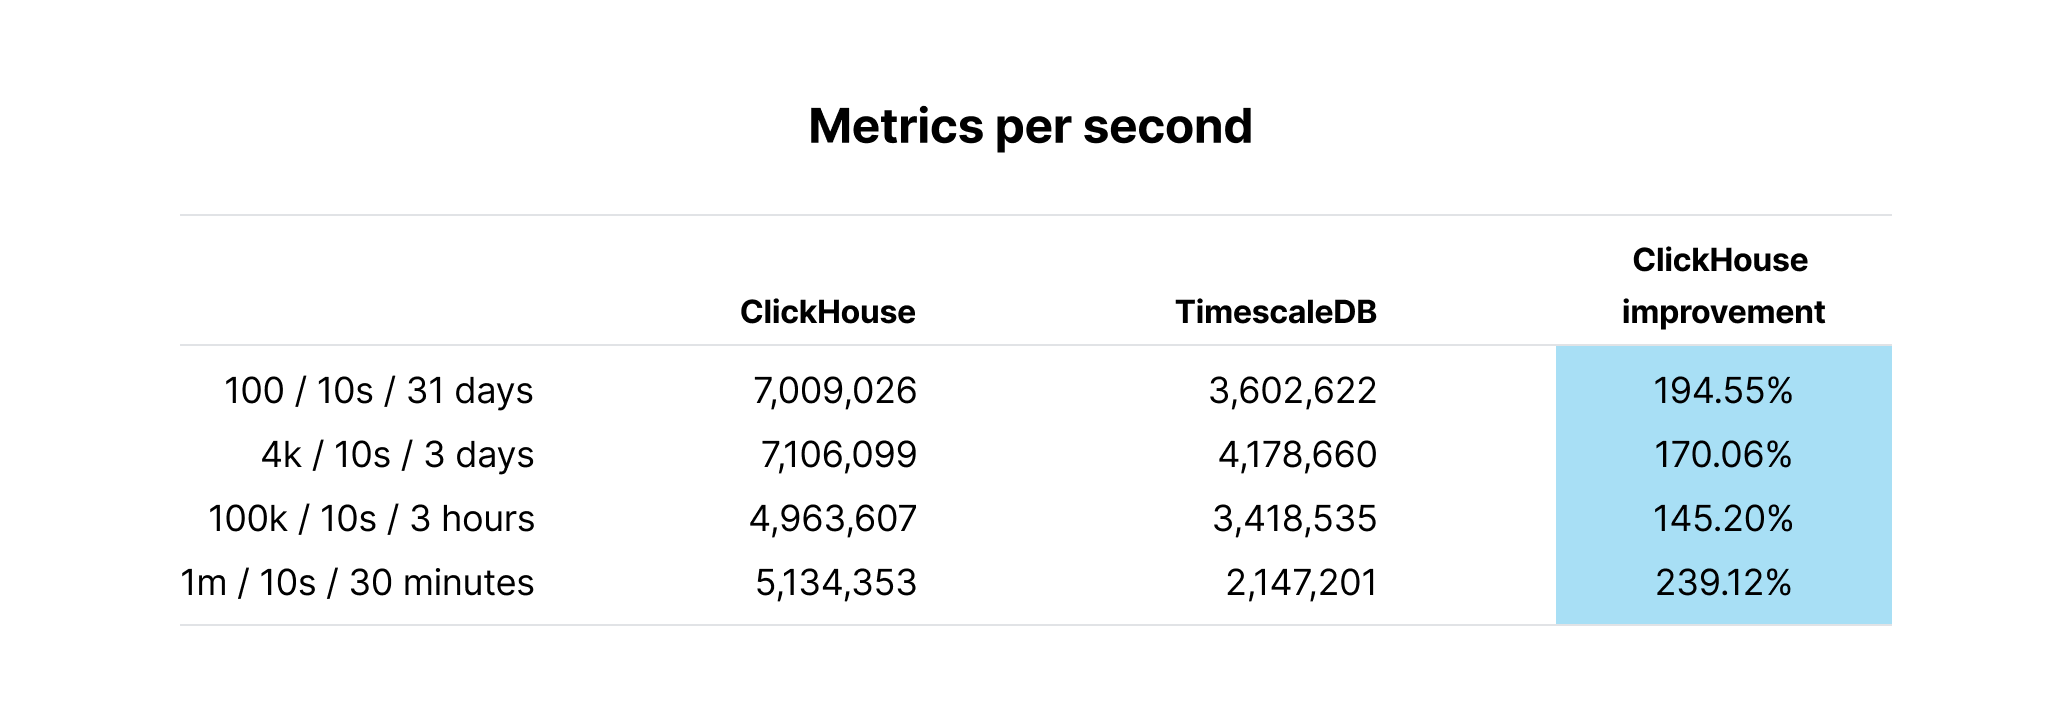
\includegraphics[width=0.85\textwidth]{imgs/07-clickhouse-improvement.png}
	\captionof{figure}{\href{https://www.timescale.com/blog/what-is-clickhouse-how-does-it-compare-to-postgresql-and-timescaledb-and-how-does-it-perform-for-time-series-data/}{Performance degli insert}}
\end{center}

\begin{center}
	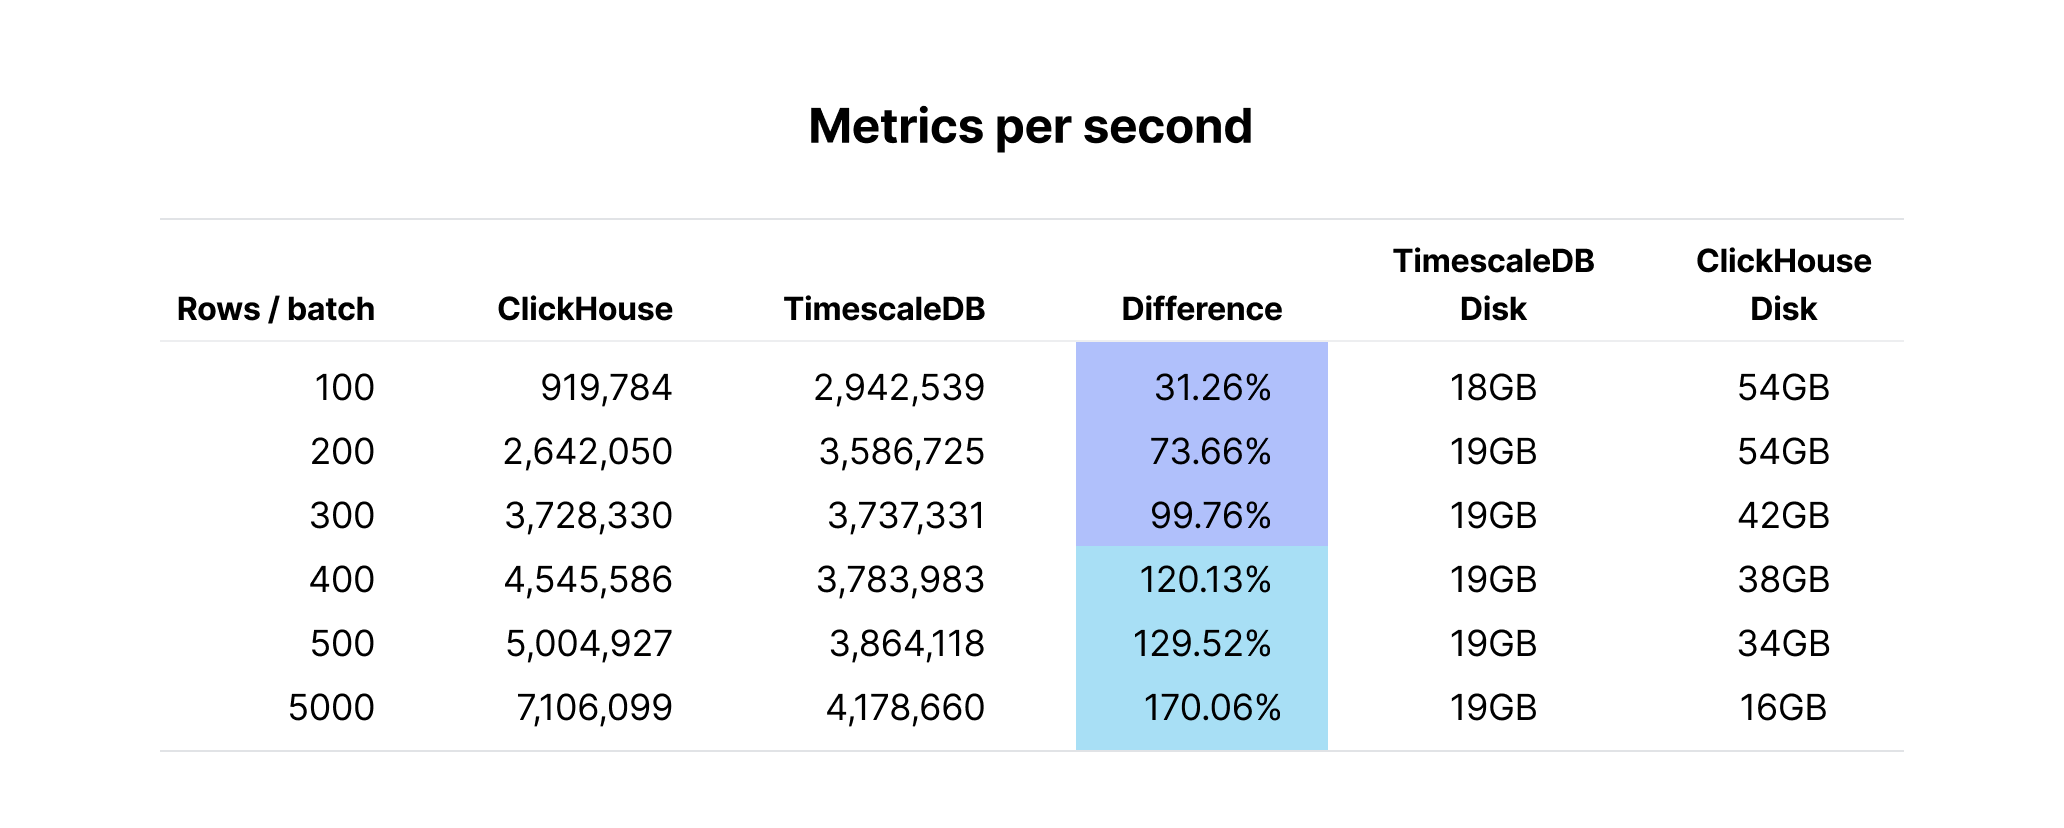
\includegraphics[width=0.85\textwidth]{imgs/08-chunk-time-interval.png}
	\captionof{figure}{\href{https://www.timescale.com/blog/what-is-clickhouse-how-does-it-compare-to-postgresql-and-timescaledb-and-how-does-it-perform-for-time-series-data/}{Performance degli insert con batch di dimensioni ridotte}}
\end{center}

\begin{center}
	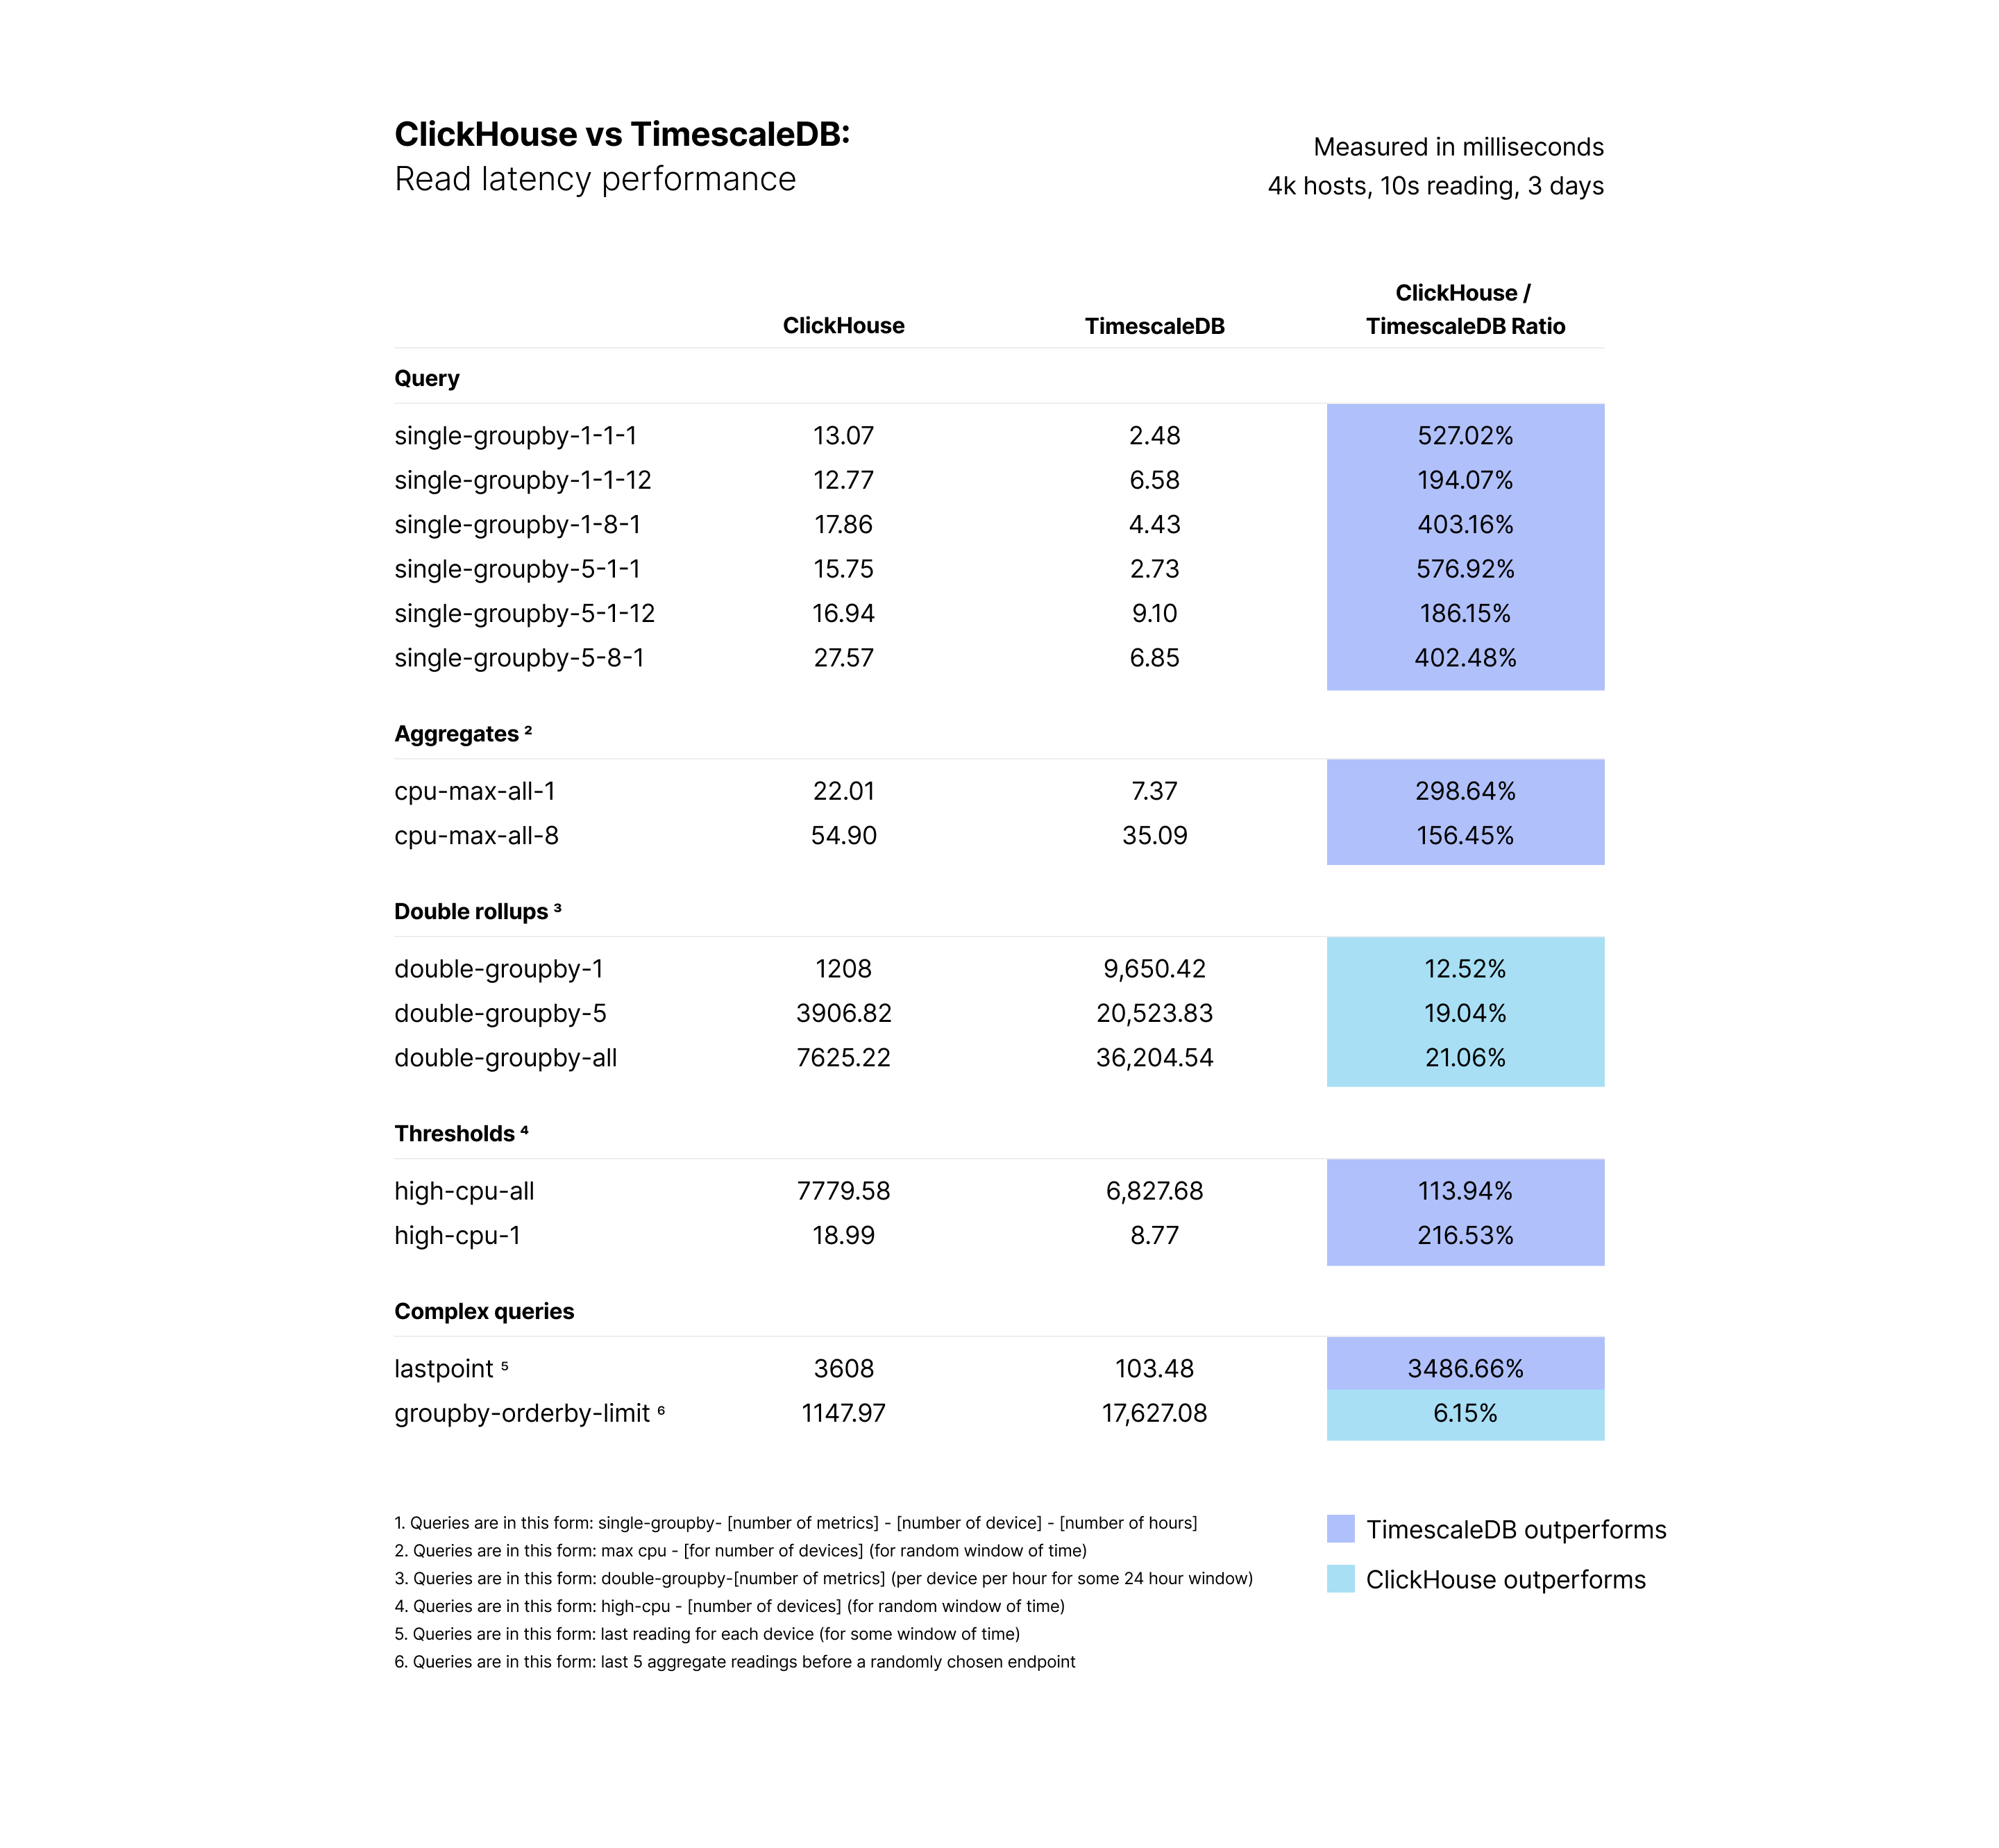
\includegraphics[width=0.85\textwidth]{imgs/09-clickhouse-benchmark-read-latency-performance.png}
	\captionof{figure}{\href{https://www.timescale.com/blog/what-is-clickhouse-how-does-it-compare-to-postgresql-and-timescaledb-and-how-does-it-perform-for-time-series-data/}{Performance di query di 4000 host con 100 milioni di righe di dati}}
\end{center}

\begin{center}
	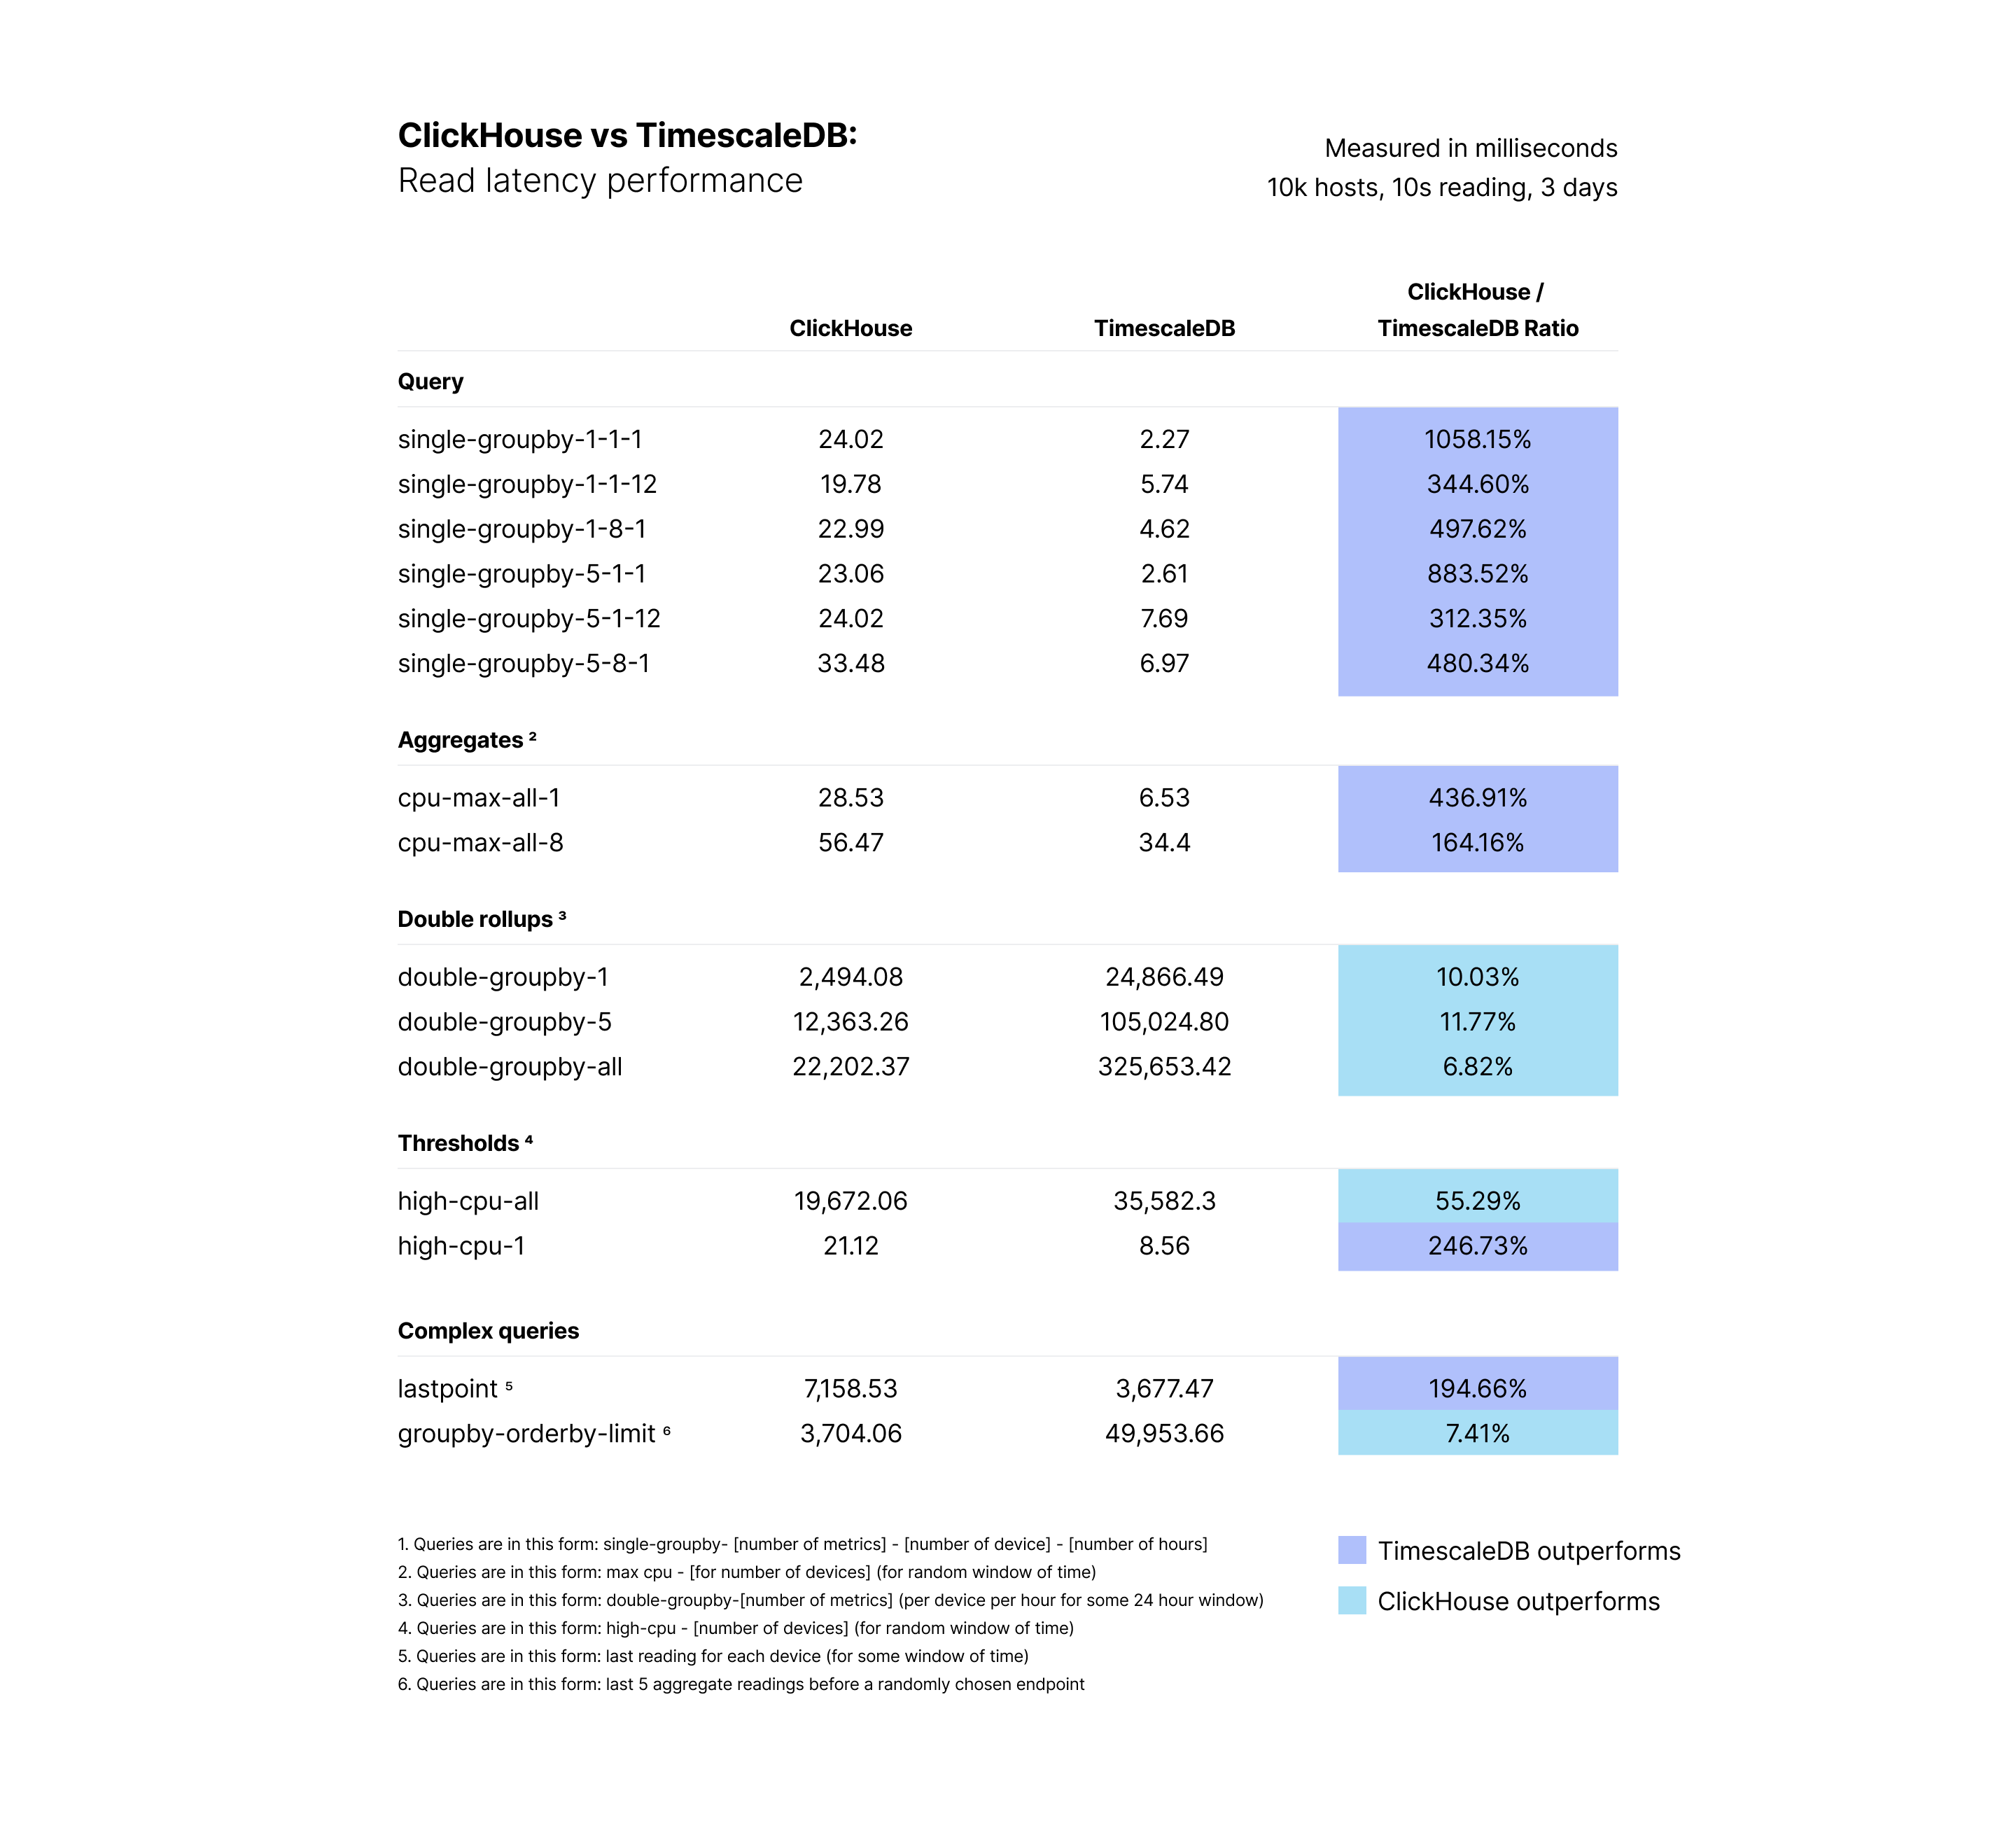
\includegraphics[width=0.85\textwidth]{imgs/10-clickhouse-benchmark-read-latency-performance.png}
	\captionof{figure}{\href{https://www.timescale.com/blog/what-is-clickhouse-how-does-it-compare-to-postgresql-and-timescaledb-and-how-does-it-perform-for-time-series-data/}{Performance di query di 10000 host con 100 milioni di righe di dati}}
\end{center}






